\thispagestyle{empty}
\section{Praktische Durchführung}
\label{Isolation Container}

In dieser Arbeit wird ausschließlich Linux verwendet, weshalb auf die Eigenschaften im Linux-Kernel eingegangen wird. In einem anderen Betriebssystem können einzelne Punkte unterschiedlich implementiert sein. Die Speicherverwaltung von Containern übernimmt das darunterliegende Betriebssystem. Weil viele Anwendungen Speicher anfragen, bevor sie diesen verwenden, wurde der Linux-Kernel mit einer \emph{Over-Commit}-Lösung ausgestattet, um Ressourcen effizient zu nutzen. Mit dieser Methode wird Speicher virtualisiert, indem Ressourcensanfragen von Anwendungen an den Betriebssystem-Kernel immer akzeptiert werden. Dadurch vergibt der Linux-Kernel mehr Speicher, als auf der Hardware tatsächlich vorhanden ist. Die Anwendungen selbst bekommen genauso viele \emph{Memory-Pages} auf der Hardware, wie aktuell benötigt werden. Mit diesem System kann es vorkommen, dass mehr Speicher benötigt wird, als physisch vorhanden ist. 

Wenn der Speicher knapp wird, ist \emph{Paging} die erste Reaktion des Betriebssystems. Beim Paging werden allokierte Memory-Pages, die aktuell nicht verwendet werden, vom Arbeitsspeicher auf den Massenspeicher geladen. Da ein Massenspeicherzugriff sehr aufwändig und langsam ist, wurde diese Möglichkeit der zusätzlichen Speichererweiterung limitiert. Auf dem in dieser Arbeit verwendetem System, liegt das Limit bei 2 GB. Wenn Paging nicht ausreicht, wird der \ac{OOM-Killer} aufgerufen. Der OOM-Killer beendet anhand einer Prioritätenliste die niederwertigsten Prozesse, bis ausreichend Platz geschaffen wurde. Jeder Prozess erhält bereits bei der Erstellung eine Priorisierung in Form einer Zahl, die nach Eigenschaft und Wichtigkeit die Priorität widerspiegelt.

Bei der Erstellung von Containern wird ein in der maximalen Größe definierter, durch Cgroup beschränkter und durch Namespace isolierter Bereich geschaffen. Die aktuelle Größe des Bereichs hängt von den aktuell verwendeten Ressourcen ab und liegt im Regelfall unter der maximalen Begrenzung. Mehrere voneinander gut isolierte Container teilen sich ein durch das Betriebssystem verwaltetes Hardwaresystem. Wegen der Speicherverwaltung des Linux-Kernels ist es möglich, dass ein Container Einfluss auf einen anderen Container nehmen kann. Durch einen erhöhten Speicherverbrauch kann ein Container mit Hilfe des OOM-Killers Einfluss auf einen anderen Container nehmen. Somit sind Container nicht vollständig isoliert.

\subsection{Hardware und Software}

Das gerade beschriebene Szenario soll im praktischen Teil dieser Arbeit untersucht werden. \textcolor{magenta}{Das daraus resultierende Ergebnis wird im letzten Abschnitt mit dem Hypervisor-Virtualisierungsansatz verglichen.} Als Container-basierte Virtualisierungslösung wurde Docker ausgewählt. Docker ist aktuell die am weitesten verbreitete Softwarelösung für die Erstellung von Containern und basiert auf dem Prinzip der Linux-Container (LXC).

\textcolor{magenta}{Hier will noch Details über die Hardware rein.}



\subsection{Docker}
Die Docker-Container Technologie wurde 2013 als das Open Source Projekt unter dem Namen \emph{Docker Engine} eingeführt. Basierend auf Linux-Container-Konzepten nutzt auch Docker Namespaces und Cgroups zur Isolierung und Limitierung von Containern.  

\subparagraph{Docker-Engine}
Docker ist eine client-server Applikation. Der Docker-Client kommuniziert mit dem Docker Server, auch bekannt als Docker-Deamon oder Docker-Engine, der den Großteil der Arbeit übernimmt. Es ist möglich den Docker-Deamon und den Docker-Client auf demselben Host laufen zu lassen oder den lokalen Docker-Client mit dem Docker-Deamon auf einem anderen Host zu verbinden. Die Docker-Architektur ist in Abbildung \ref{fig:Docker_Server_Client.PNG} dargestellt \cite{Turnbull2015TheBook}.

\vspace{1em}
\begin{minipage}{\linewidth}
	\centering
	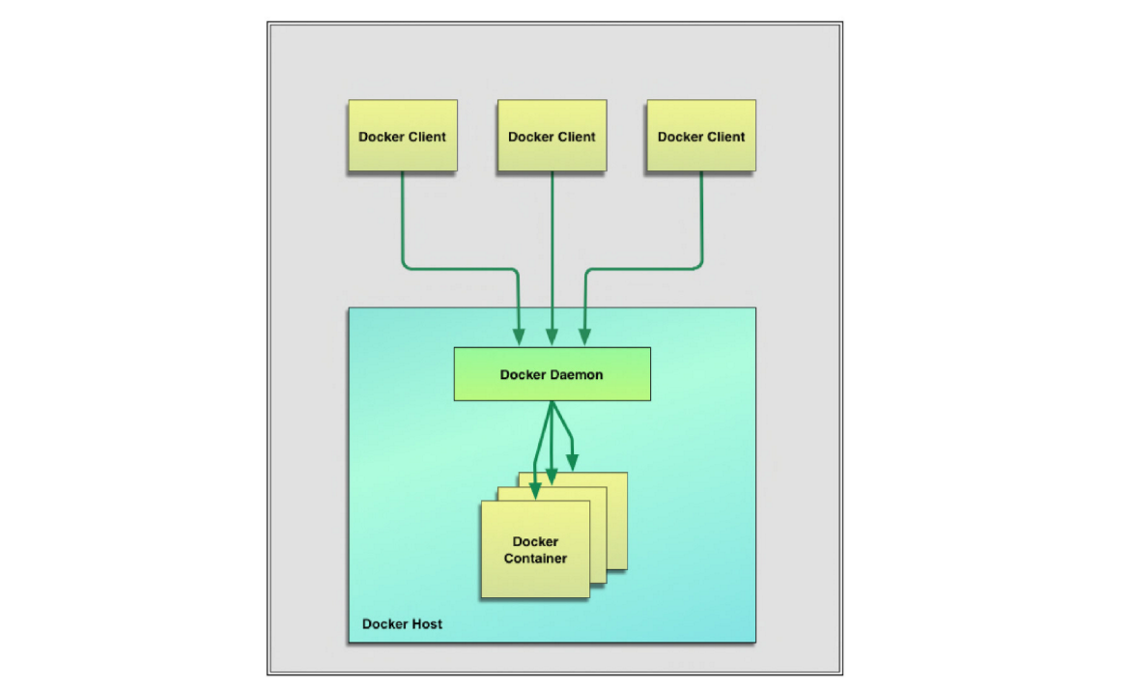
\includegraphics[width=1\linewidth]{pics/Docker_Server_Client.PNG}
	\captionof{figure}[Docker-Architektur\cite{Turnbull2015TheBook}]{Docker Architektur}
	\label{fig:Docker_Server_Client.PNG}
\end{minipage}


\subparagraph{Docker-Images}
Images sind die Bausteine der Docker Welt. Container werden von Images gestartet. Images sind ein mehrschichtiges Format, die unter Verwendung von Union-Dateisystemen Schritt für Schritt anhand unterschiedlicher Instruktionen erstellt werden. Diese Instruktionen können als Quellcode der Container betrachtet werden. Sie sind einfach verschiebbar und können in \emph{Registries} verwaltet werden.

\subparagraph{Registries}
Docker speichert die erstellten Images in Registries Es gibt zwei Arten von Registries: Öffentliche und private. Docker verwaltet die öffentlichen Images im Docker-Hub \cite{DockerInc.2016DockerHub}. Auf Docker-Hub können eigene Images abgespeichert und geteilt werden. Diese Plattform beinhaltet bereits zehntausende Images, die von anderen Leuten erstellt wurden und für eigene Verwendungen zur Verfügung stehen. Private Images kann man ebenfalls auf Docker-Hub abspeichern und niemand außer einem ausgewählten Personenkreis hat Zugriff darauf.

\subparagraph{Docker-Container}
Docker unterstützt den Benutzer beim Erstellen und Ausführen von Containern. Container werden von Images ausgeführt und können einen oder mehrere Prozesse beinhalten. Images können als der Aufbauprozess von Docker gesehen werden und Container als die ausführende Instanz von Docker.

Docker leiht sich das Konzept des Schiffcontainers, die für den Transport von Waren eingesetzt werden. Es dient als Modell für Docker-Container, mit dem Unterschied, dass Docker-Container keine Waren, sondern Software transportieren. Container können in jeglicher Umgebung ausgeführt werden. Ob auf dem Laptop, nach dem Download von Docker-Hub auf einem Web-, einem Datenbank- oder auf einem Applikationsserver, die Container werden geladen, wie jeder andere Container auch.

\subsection{Realisierung}
Das anfangs in diesem Kapitel genannte Szenario wird in Teilprobleme zerlegt und schrittweise zusammengefügt. Im ersten Schritt soll gezeigt werden, wie sich der Ressourcenverbrauch eines Containers erhöht und wo eventuelle Grenzen der verwendeten Hardware liegen. Im Linux-Filesystem ist es möglich, über die PID eines vorhandenen Prozesses die Cgroup herauszufinden, zu der ein Prozess gehört. Zur Erinnerung, jede Cgroup ist für die Ressourcenbegrenzung, Priorisierung, Abrechnung und Kontrolle aller Prozesse zuständig, die unter ihr erstellt wurden. Unter einem Kontrollregister im Linux-Kernel kann die Summe der verwendeten Ressourcen aller unter einer Cgroup laufenden Prozesse zur Laufzeit ausgelesen werden. Zur Durchführung wird ein neuer Docker-Container erstellt. In diesem ruft ein Programm in Endlosschleife den malloc() Befehl auf. Dieses Programm wurde in der Programmiersprache \emph{C} erstellt. Mit Hilfe der Cgroup wird der Speicherverbrauch des Containers überwacht.

\subparagraph{Test01}
Auf Docker-Hub wird ein geeignetes Image ausgesucht und für den Test erweitert. Beim Ausführen des Images wird ein Docker-Container erstellt. Ressourcenlimits können ebenfalls vor dem Starten des Containers eingestellt werden. Für den ersten Start sind allerdings noch keine Begrenzungen des Speichers nötig, da es in erster Linie um die Auswirkung des ausgeführten C-Programms auf die Ressourcenverwaltung im Container geht. Der verwendete C-Code, den der Prozess ausführt, ist in Listing \ref{01mem} zu sehen. Ein erstelltes Skript verwendet die beim Start erzeugte PID, findet die Cgroup in der der Prozess ausgeführt wird und schreibt die ausgelesenen Messdaten in eine Text-Datei. Die Messdaten wie System-Clock-Time in Nanosekunden und Speicherverbrauch in Bytes werden für die Auswertung verwendet.


\vspace{1em}
\lstinputlisting[caption=malloc()-Befehl in Endlosschleife, label=01mem, basicstyle=\ttfamily\scriptsize]{code/01mem.txt}

\subparagraph{Erwartungshaltung Test01}
Unter der Annahme, dass das Skript die Messwerte in ungefähr gleichmäßigen Abständen liefert, wird ein linearer Zusammenhang zwischen Zeit und Speicherverbrauch erwartet. Dazu muss die Speicheralokation in jedem Durchlauf stets eine vergleichbare Zeit in Anspruch nehmen. Wenn nicht mehr genug Speicher im System vorhanden ist, wird der OOM-Killer den Prozess beenden.

\vspace{2em}
\begin{minipage}{\linewidth}
	\centering
	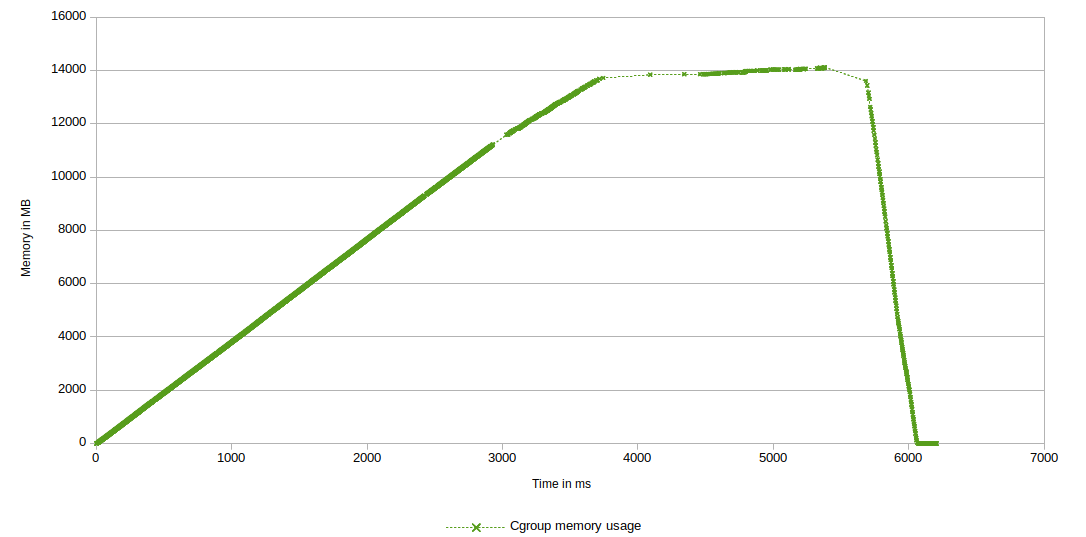
\includegraphics[width=1\linewidth]{pics/001_mem_usage_No_Limit_Cgroup_RDY_FOR_USE.png}
	\captionof{figure}[Speicher Verbrauch Cgroup Ohne Limit]{Endlosschleife malloc(), Speicherverbrauch einer Cgroup ohne Limit}
	\label{fig:001_mem_usage_No_Limit_Cgroup_RDY_FOR_USE}
\end{minipage}


\subparagraph{Ergebnis Test01}
In Abbildung \ref{fig:001_mem_usage_No_Limit_Cgroup_RDY_FOR_USE} ist wie erwartet ein linearer Zusammenhang erkennbar. Bei ca. \SI{13900}{\mega\byte} allokiertem Speicher sättigt die Kurve. An diesem Punkt ist der insgesamt \SI{16}{\giga\byte} große Arbeitsspeicher größtenteils ausgeschöpft. Ein paar Megabyte konnten vom Betriebssystem für den dauerhaft nach mehr Speicher verlangendem Prozess gefunden werden. Bei knapp über \SI{14000}{\mega\byte} wurde der OOM-Killer eingeschaltet, um wichtigere Prozesse zu schützen und der Container wurde beendet.

\subparagraph{Test02}
Im nächsten Schritt wird der Verlauf einer Cgroup näher betrachtet, bei der ein willkprliches Speicherlimit festlegt wird, das nicht überschritten werden soll (Hard-Limit). Um dieses Limit zu erstellen, wird das Image entsprechend angepasst und das Speicherlimit auf \SI{8200}{\mega\byte} gesetzt. Das in Listing \ref{01mem} vorgestellte Programm wird wieder ausgeführt.

\subparagraph{Erwartungshaltung Test02}
Da nun ein Hard-Limit eingerichtet ist, wird die Cgroup mit der gleichen Geschwindigkeit wie in Abbildung \ref{fig:001_mem_usage_No_Limit_Cgroup_RDY_FOR_USE} bis zum gesetzten Limit ansteigen und dieses nicht überschreiten. 

\vspace{1em}
\begin{minipage}{\linewidth}
	\centering
	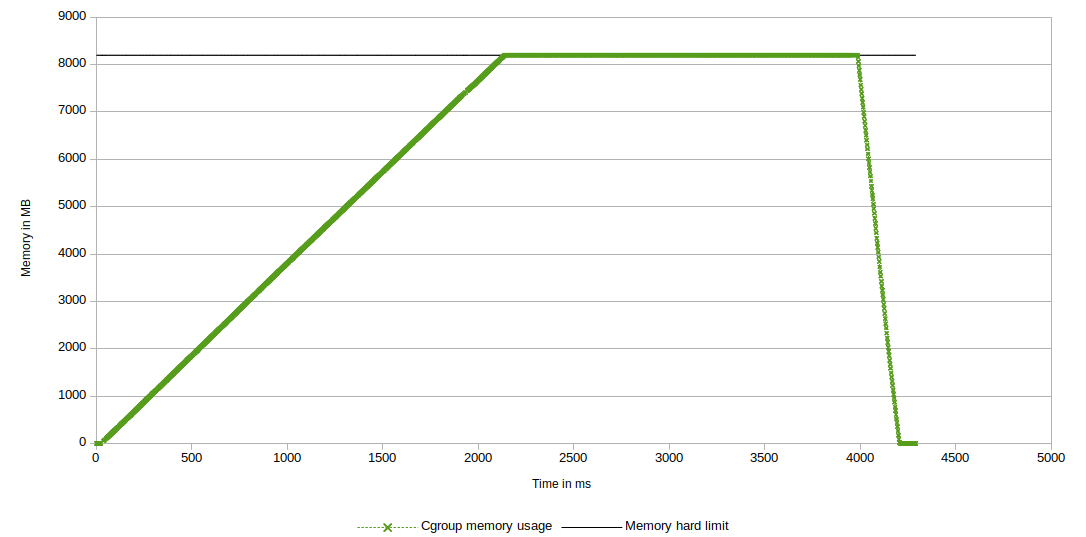
\includegraphics[width=1\linewidth]{pics/002_mem_usage_8200mb_limit_Cgroup_RDY_FOR_USE.png}
	\captionof{figure}[Speicher Verbrauch Cgroup 8200MB Limit]{Endlosschleife malloc(), Speicherverbrauch einer Cgroup mit Limit}
	\label{fig:002_mem_usage_8200mb_limit_Cgroup_RDY_FOR_USE}
\end{minipage}

\subparagraph{Ergebnis Test02}
Mit einer Allokationsrate von ca. \SI{4000}{\mega\byte\per\second} ändert sich die Speicherzugriffsrate nicht. Das Limit von \SI{8200}{\mega\byte} wurde erfolgreich eingehalten und der Prozess später vom Betriebssystem beendet.

In den Abbildungen \ref{fig:001_mem_usage_No_Limit_Cgroup_RDY_FOR_USE} und \ref{fig:002_mem_usage_8200mb_limit_Cgroup_RDY_FOR_USE} tritt eine Sättigung der Speicherallokation ein. Es stellt sich die Frage, warum das Programm nicht zum Zeitpunkt der Sättigung, sondern erst zu einem späteren Zeitpunkt vom OOM-Killer beendet wird. Das legt den Schluss nahe, dass das Programm weiterhin Speicher vom Betriebssystem erhält, die Cgroup jedoch nicht in der Lage ist, dies zu erfassen. 

Betrachtet man die Cgroup wie eine Box, ist eine mögliche Erklärung für das oben gezeigte Verhalten herleitbar. Die Größe der Box wird bei der Erstellung des Containers festgelegt. In Abbildung \ref{fig:002_mem_usage_8200mb_limit_Cgroup_RDY_FOR_USE} waren es \SI{8200}{\mega\byte}. Der Füllstand der Box setzt sich aus den verwendeten Ressourcen aller in der Box ausgeführten Prozesse zusammen. Wenn ein Prozess wie in Abbildung \ref{fig:002_mem_usage_8200mb_limit_Cgroup_RDY_FOR_USE} die komplette Box ausfüllt und weiter darüber hinaus ragen würde, wäre die Box nur in der Lage den Füllstand bis zu Ihrer Maximalgröße von \SI{8200}{\mega\byte} widerzuspiegeln. Der überlaufende Teil des Prozesses kann von der Cgroup nicht erkannt werden.

\subparagraph{Test03}
Nach oben genannter Vermutung liegt es nun nahe, den Speicherverbrauch des Prozesses genauer zu untersuchen. Das Testskript wird erweitert, um die vom Prozess verwendete Anzahl der Memory-Pages auszugeben. Die Anzahl an benötigten Memory-Pages in einem laufenden Prozess, kann ebenfalls im Linux-Kernel ausgelesen werden. Eine Memory-Page ist \SI{4}{\kilo\byte} groß und ergibt multipliziert mit der verwendeten Anzahl an Memory-Pages den Speicherverbrauch.

\subparagraph{Erwartungshaltung Test03}
Wenn die Memory-Page Größe multipliziert mit der Anzahl der verwendeten Memory-Pages genau dem entspricht, was die Cgroup an Speicherallokation ausgibt, sollten beide Graphen bis zum Erreichen des Limits deckungsgleich sein.

\vspace{1em}
\begin{minipage}{\linewidth}
	\centering
	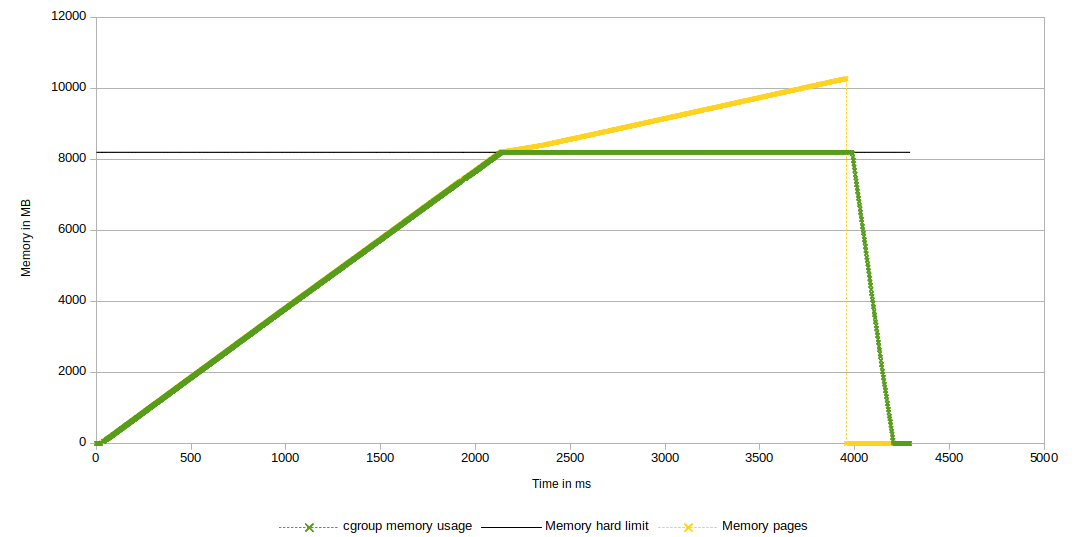
\includegraphics[width=1\linewidth]{pics/003_mem_usage_8200mb_limit_Cgroup_Pages_RDY_FOR_USE.png}
	\captionof{figure}[ Endlosschleife Malloc]{Endlosschleife malloc(), Speicherverbrauch einer Cgroup und Memory-Pages mit Limit}
	\label{fig:003_mem_usage_8200mb_limit_Cgroup_Pages_RDY_FOR_USE}
\end{minipage}

\subparagraph{Ergebnis Test03}
Deutlich in Abbildung \ref{fig:003_mem_usage_8200mb_limit_Cgroup_Pages_RDY_FOR_USE} zu erkennen sind die exakt aufeinanderliegenden Messwerte der Cgroup und der Memory-Pages. Ab \SI{8200}{\mega\byte} überschreiten die allokierten Memory Pages bis ca. \SI{10200}{\mega\byte} das Limit. Erkennbar ist auch die geringere Allokationsrate die nach dem Überlauf auf \SI{2000}{\mega\byte\per\second} fällt. Komplett ignoriert wurde das Limit allerdings nicht. Verglichen mit Abbildung \ref{fig:001_mem_usage_No_Limit_Cgroup_RDY_FOR_USE} war noch genügend Speicher im System vorhanden. Somit stellen sich folgende Fragen:

\begin{itemize}
    \item Wieso wurde der Prozess dann überhaupt schon beendet?
    \item Warum konnte er über das Limit hinaus allokieren? 
    \item Wie verhält sich ein Container, wenn er nur ein wenig über das Limit geht?
    \item Wie wirkt sich das auf andere Container im System aus?
\end{itemize}


Eine mögliche Antwort ist das Paging. Beim Paging werden allokierte, aber aktuell nicht verwendete Memory-Pages vom Arbeitsspeicher auf den Massenspeicher geladen. In Abbildung \ref{fig:003_mem_usage_8200mb_limit_Cgroup_Pages_RDY_FOR_USE} ist nach \SI{8200}{\mega\byte} die Trennung zwischen der gelben Linie (Memory-Page) und der grünen Linie (Cgroup) zu erkennen. Zu diesem Zeitpunkt hat das Betriebssystem mit dem Paging begonnen und lädt von dem Prozess allokierte Pages in den Massenspeicher. Die tatsächliche Menge an Arbeitsspeicher, der von der Cgroup auf der Hardware allokiert ist, bleibt gleich. Die gelbe Linie zeigt die Summe aller vom Prozess allokierten Memory-Pages, folglich auch den auf den Massenspeicher ausgelagerten Anteil. Die Steigung der gelben Linie ist durch die erhöhten Anforderungen an das I/O-System, was das Paging zu verantworten hat, zu erklären. Deshalb verringert sich die Allokationsrate beim Überschreiten des Limits. Der Überlauf von ca. \SI{2}{\giga\byte} stimmt mit dem \SI{2}{\giga\byte} Paging-Limit überein.

\subparagraph{Test03,5}
Zur Abklärung und Überprüfung des Paging-Limits empfiehlt es sich, den Test01  zu wiederholen und zusätzlich die Memory-Pages zu betrachten.

\subparagraph{Erwartungshaltung Test03,5}
Es wurden ca. \SI{14000}{\mega\byte} beim ersten Testdurchlauf allokiert. Mit dem zusätzlichen Paging-Limit von \SI{2}{\giga\byte} sind die Memory-Pages auf ca. \SI{16000}{\mega\byte} zu schätzen. Ein identischer Cgroup Graph wird nicht erwartet, da der Arbeitsspeicherverbrauch des Betriebssystems von mehreren Faktoren abhängt. Doch der Unterschied zwischen dem Speicherverbrauch der Cgroup und den Memory-Pages sollte bei etwa \SI{2}{\giga\byte} liegen. 

\vspace{1em}
\begin{minipage}{\linewidth}
	\centering
	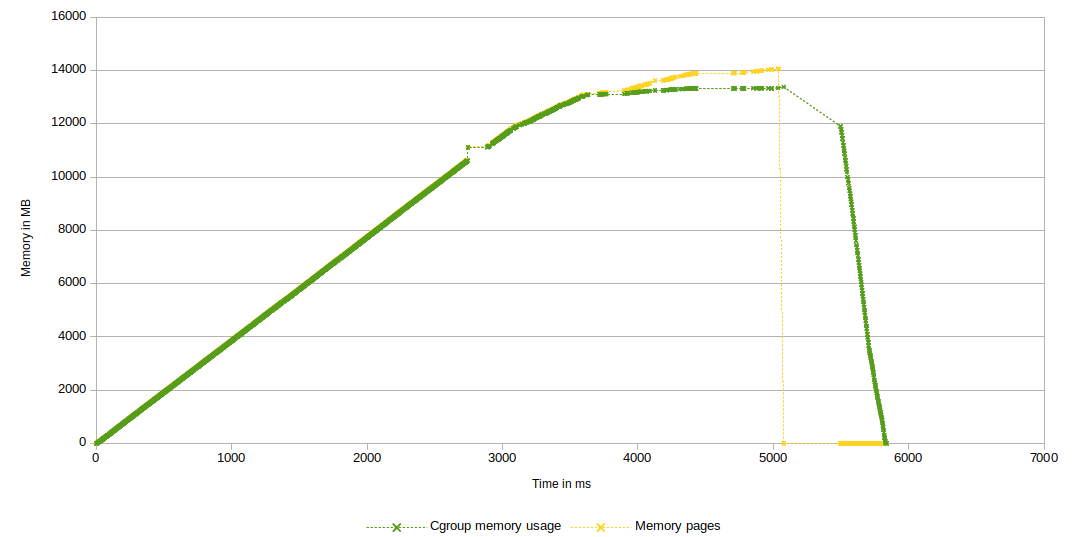
\includegraphics[width=1\linewidth]{pics/001,5_mem_usage_No_Limit_Cgroup_Pages_RDY_FOR_USE.png}
	\captionof{figure}[Speicher Verbrauch Cgroup 8200MB Limit]{Endlosschleife malloc(), Speicherverbrauch einer Cgroup und Memory-Pages ohne Limit}
	\label{fig:001,5_mem_usage_No_Limit_Cgroup_Pages_RDY_FOR_USE.png}
\end{minipage}

\subparagraph{Ergebnis Test03,5}
In Abbildung \ref{fig:001,5_mem_usage_No_Limit_Cgroup_Pages_RDY_FOR_USE.png} sind die \SI{2}{\giga\byte} Unterschied zwischen dem Speicherverbrauch der Cgroup und den Memory-Pages offensichtlich nicht erreicht worden, was mehrere Gründe haben kann. Möglich ist eine zusätzliche Speicheranforderung des Betriebssystems, während der Prozess in der Paging-Phase war und zum früheren Absturz geführt hat. Auf diesen Effekt wird im Rahmen dieser Arbeit nicht genauer eingegangen.



\subparagraph{Test04}
In einem weiteren Schritt wird nun ein Container erstellt, der für eine gewisse Zeitspanne läuft. Das in Listing \ref{01mem} gezeigte Programm wird so modifiziert, dass das gesetzte Limit knapp überschritten wird und ist in Listing \ref{02mem} zu sehen. 

\vspace{1em}
\lstinputlisting[caption=malloc()-Befehl \SI{2200000}{mal}, label=02mem, basicstyle=\ttfamily\scriptsize]{code/02mem.txt}

\subparagraph{Erwartungshaltung Test04}
Nachdem der malloc() Befehl jetzt \SI{2200000}{mal} ausgeführt wird, sollte der Speicherverbrauch der Memory-Pages nicht über \SI{8600}{\mega\byte} steigen und \SI{60}{\second} diesen Wert halten.



\[\mathrm{sizeof(int)} = \SI{4}{\byte}\]

\[\mathrm{sizeof(int)} * \SI{1024}{} = \SI{4}{\kilo\byte}\]

\[\mathrm{sizeof(int)} * \SI{1024}{} * \SI{2200000}{} \approx \SI{8600}{\mega\byte} \]


\vspace{1em}
\begin{minipage}{\linewidth}
	\centering
	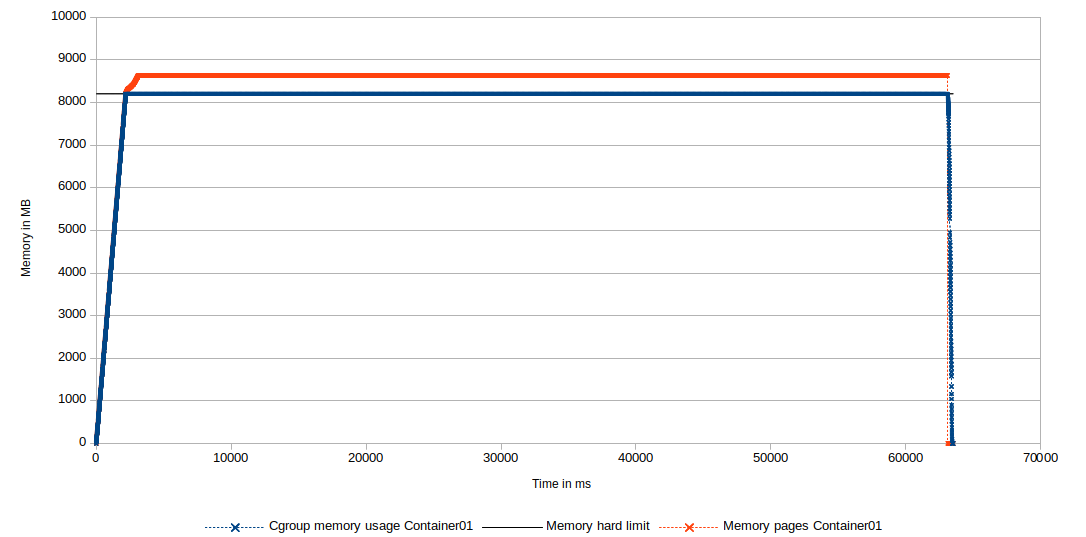
\includegraphics[width=1\linewidth]{pics/004_mem_usage_8200mb_limit_Container01_Basis_RDY_FOR_USE.png}
	\captionof{figure}[Speicher Verbrauch Cgroup 8200MB Limit]{\SI{2200000}{mal} malloc(), \SI{60}{\second} sleep(), Speicherverbrauch einer Cgroup und Memory-Pages mit Limit}
	\label{fig:004_mem_usage_8200mb_limit_Container01_Basis_RDY_FOR_USE}
\end{minipage}

\subparagraph{Ergebnis Test04}
Wie in Abbildung \ref{fig:004_mem_usage_8200mb_limit_Container01_Basis_RDY_FOR_USE} zu entnehmen, ist es möglich für einen längeren Zeitraum über das Limit hinaus Ressourcen zu allokieren. Durch die lange Ausführungszeit mit gleichbleibenden Ressourcen ist es jetzt möglich, den Einfluss von Containern untereinander zu untersuchen. Dieser Container wird von nun an als Container01 bezeichnet.

\subparagraph{Test05}
Als Container02 wird im Folgenden der Container aus Test03 bezeichnet. Im Ablauf des folgenden Tests wird zuerst Container01 gestartet und während der Laufzeit wird Container02 ebenfalls eingeschaltet. Der Container02 wird zum besseren Verständnis in Abbildung \ref{fig:005_mem_usage_8200mb_limit_Container02_Basis_RDY_FOR_USE_FOCUS} nochmals mit der gleichen Zeitachse wie in Abbildung \ref{fig:004_mem_usage_8200mb_limit_Container01_Basis_RDY_FOR_USE} dargestellt. 


\vspace{1em}
\begin{minipage}{\linewidth}
	\centering
	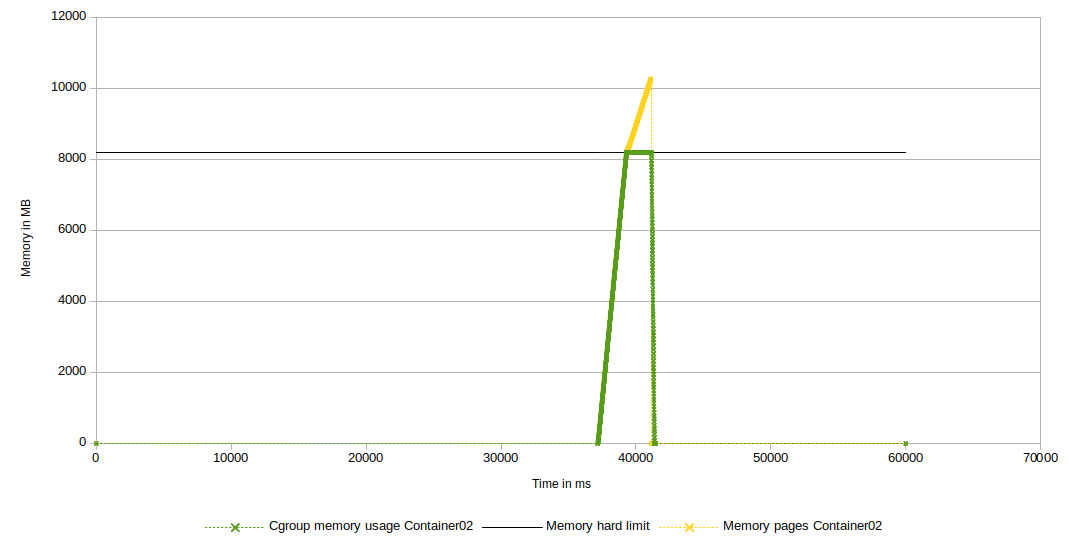
\includegraphics[width=1\linewidth]{pics/005_mem_usage_8200mb_limit_Container02_Basis_RDY_FOR_USE_FOCUS.png}
	\captionof{figure}[Speicher Verbrauch Cgroup 8200MB Limit]{Endlosschleife malloc(), Speicherverbrauch einer Cgroup und Memory-Pages mit Limit, angepasste Zeitachse}
	\label{fig:005_mem_usage_8200mb_limit_Container02_Basis_RDY_FOR_USE_FOCUS}
\end{minipage}

\subparagraph{Erwartungshaltung Test05}
Die verwendbaren Systemressourcen liegen nach Abbildung \ref{fig:001_mem_usage_No_Limit_Cgroup_RDY_FOR_USE} bei etwa \SI{14000}{\mega\byte}. Allein Container01 verwendet schon ca. \SI{8600}{\mega\byte} der gesamten Summe, was die Deckelung von Container02 auf \SI{8200}{\mega\byte} rein rechnerisch unnötig macht. Somit wird Container02 frühzeitig beendet. 

\vspace{1em}
\begin{minipage}{\linewidth}
	\centering
	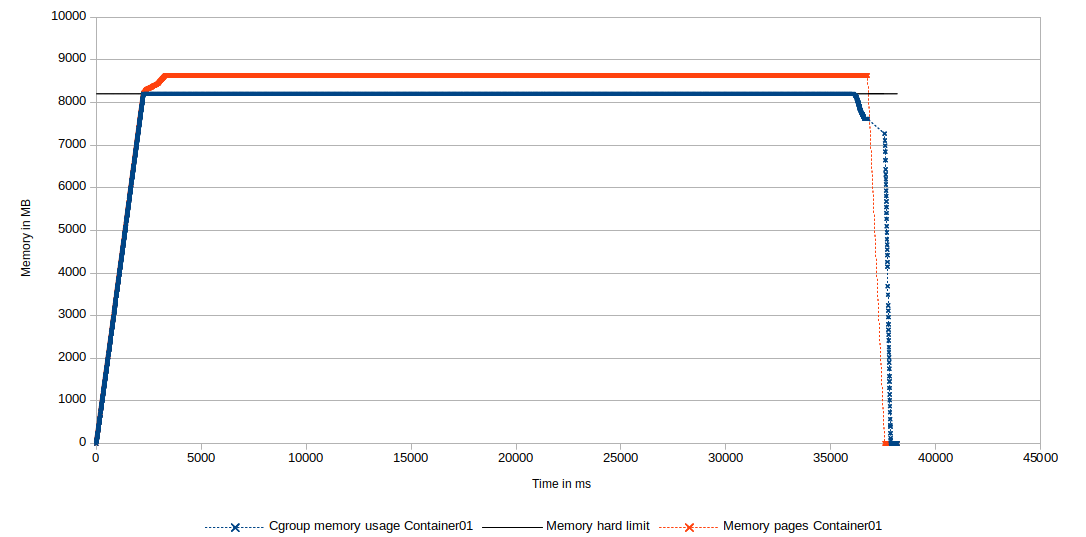
\includegraphics[width=1\linewidth]{pics/006_mem_usage_8200mb_limit_Container01_mit_ipact_RDY_FOR_USE.png}
	\captionof{figure}[Speicher Verbrauch Cgroup 8200MB Limit]{\SI{2200000}{mal} malloc(), \SI{60}{\second} sleep(), Speicherverbrauch einer Cgroup und Memory-Pages mit Limit, frühzeitiger Abbruch}
	\label{fig:006_mem_usage_8200mb_limit_Container01_mit_ipact_RDY_FOR_USE}
\end{minipage}

\subparagraph{Ergebnis Test05}
In Abbildung \ref{fig:006_mem_usage_8200mb_limit_Container01_mit_ipact_RDY_FOR_USE} ist zu erkennen, dass Container01 nicht nach ca. \SI{63}{\second} geplant beendet wurde, sondern schon etwa nach ca. \SI{38}{\second}.

Abbildung \ref{fig:007_mem_usage_8200mb_limit_Container01_und_Container02_RDY_FOR_USE} zeigt beide Container mit einer gemeinsamen Zeitachse. Nach dem Start von Container02, als dieser ca. \SI{5100}{\mega\byte} Speicher allokiert hat, wird Container01 beendet. Container02 überschreitet das Limit von \SI{8200}{\mega\byte} nach ca. \SI{41}{\second} und wird nach ca. \SI{42,5}{\second} ebenfalls beendet.

\vspace{1em}
\begin{minipage}{\linewidth}
	\centering
	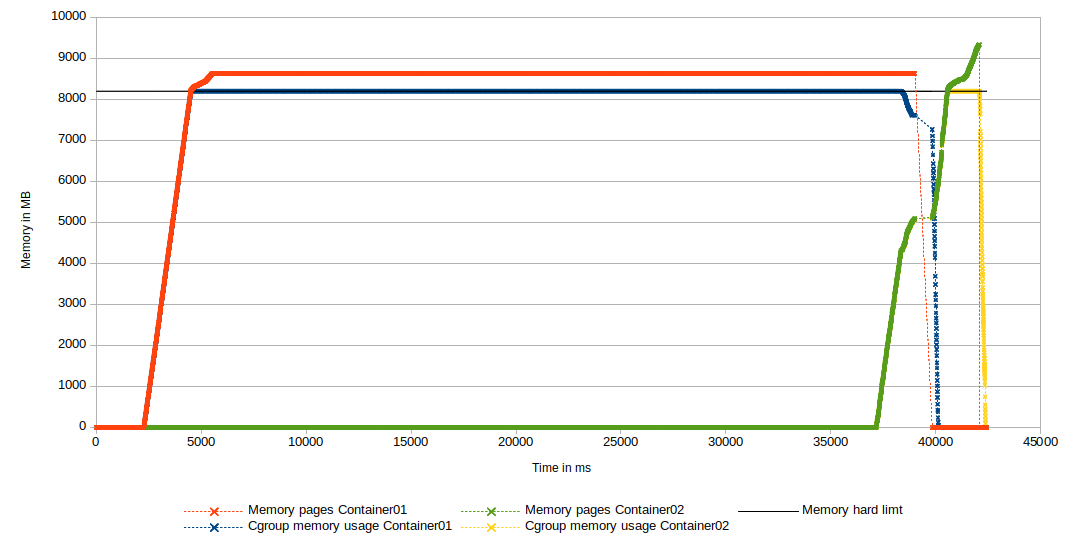
\includegraphics[width=1\linewidth]{pics/007_mem_usage_8200mb_limit_Container01_und_Container02_RDY_FOR_USE.png}
	\captionof{figure}[Speicher Verbrauch Cgroup 8200MB Limit]{Speicherverbrauch einer Cgroup und Memory-Pages mit Limit von Container01 mit \SI{2200000}{mal} malloc(), \SI{60}{\second} sleep() und von Conteiner02 mit Endlosschleife malloc()}
	\label{fig:007_mem_usage_8200mb_limit_Container01_und_Container02_RDY_FOR_USE}
\end{minipage}

Abbildung \ref{fig:008_mem_usage_8200mb_limit_Container01_und_Container02_RDY_FOR_USE_FOCUS} zeigt den interessanten Teil aus Abbildung \ref{fig:007_mem_usage_8200mb_limit_Container01_und_Container02_RDY_FOR_USE}. Am auffälligsten ist die Lücke (mit gestrichelten Linien gekennzeichnet) in der Mitte der Abbildung. Eine Lücke entsteht, wenn über mehrere Millisekunden keine Messwerte vom Skript erfasst werden können. In diesem Fall ist das auf eine Systemüberlastung zurück zu führen, welche durch die Überlastung des Arbeitsspeichers und die dadurch eingeleiteten Systemreaktionen entstanden ist. 

\vspace{1em}
\begin{minipage}{\linewidth}
	\centering
	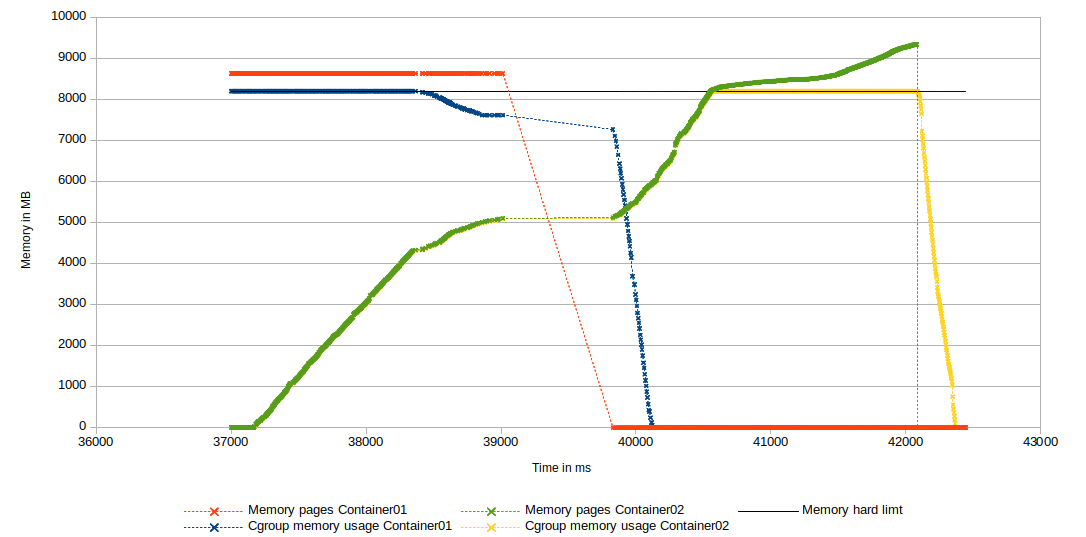
\includegraphics[width=1\linewidth]{pics/008_mem_usage_8200mb_limit_Container01_und_Container02_RDY_FOR_USE_FOCUS.png}
	\captionof{figure}[Speicher Verbrauch Cgroup 8200MB Limit]{Speicherverbrauch einer Cgroup und Memory-Pages mit Limit von Container01 mit \SI{2200000}{mal} malloc(), \SI{60}{\second} sleep() und von Conteiner02 mit Endlosschleife malloc(), Fokus}
	\label{fig:008_mem_usage_8200mb_limit_Container01_und_Container02_RDY_FOR_USE_FOCUS}
\end{minipage}



Die blauen Linie zeigt den Speicherverbrauch der Cgroup von Container01 in Abbildung \ref{fig:008_mem_usage_8200mb_limit_Container01_und_Container02_RDY_FOR_USE_FOCUS}, bei der nach ca. \SI{38,5}{\second} ein Abwärtstrend zu erkennen ist. Zu diesem Zeitpunkt hat das Betriebssystem mit dem Paging begonnen und lädt von der Cgroup allokierte Pages in den Massenspeicher. Die tatsächliche Menge an Arbeitsspeicher, welchen die Cgroup allokiert, nimmt ab. Die rote Linie zeigt die Summe aller vom Prozess allokierten Memory-Pages, folglich auch den auf den Massenspeicher ausgelagerten Anteil. Der Verlauf der grünen Linie zeigt die Memory-Pages von Container02 und lässt sich durch folgende Annahme begründen. Wegen der erhöhten Anforderung an das I/O-System, welche das Paging zu verantworten hat, verringert sich die Allokationsrate. Nach dem Beenden von Container01 wird ebenfalls das Paging beendet. Dadurch verläuft die Steigung der Kurve von Container02 ähnlich wie nach dem Start des Prozesses. 

\subparagraph{Test06}
Bisher wurden Container betrachtet, die sich nicht an das vorgegebene Limit gehalten haben. Im Folgenden gilt es zu zeigen, dass auch bei \glqq gutartigen\grqq{}  Containern, also Container welche sich immer unter dem vorgegebenen Limit befinden, ähnliche Effekte auftreten. Für den folgenden Testdurchlauf wird der in Listing \ref{03mem} gezeigte C-Code verwendet. Zuerst startet Container03, der den eben genannten C-Code ausführt. Während des \SI{60}{\second} sleep() startet Container04 ebenfalls mit dem in Container03 verwendeten Code.

\vspace{1em}
\lstinputlisting[caption=einfacher C-Code, label=03mem, basicstyle=\ttfamily\scriptsize]{code/03mem.txt}

\subparagraph{Erwartungshaltung Test06}
Durch die Änderung auf \SI{2048000}{} Wiederholungen des malloc()-Befehls, wird Container03 bis ca. \SI{8000}{\mega\byte} Speicher allokieren. Nach dem Start von Container04 wird ein ähnlicher Graphenverlauf erwartet wie im vorherigen Test. Da das gesetzte Hard Limit bei \SI{8200}{\mega\byte} nicht überschritten wird, werden die Linien der Cgroup und der Memory-Pages von Container04 identisch über die Lebensdauer des Containers verlaufen.

\[\mathrm{sizeof(int)} = \SI{4}{\byte}\]

\[\mathrm{sizeof(int)} * \SI{1024}{} = \SI{4}{\kilo\byte}\]

\[\mathrm{sizeof(int)} * \SI{1024}{} * \SI{2048000}{} \approx \SI{8000}{\mega\byte} \]

\vspace{1em}
\begin{minipage}{\linewidth}
	\centering
	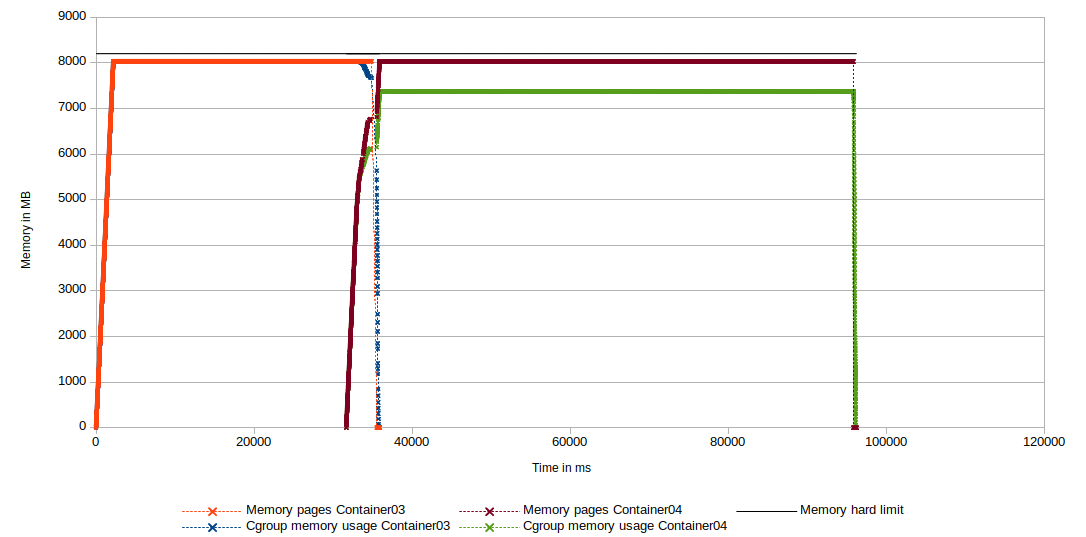
\includegraphics[width=1\linewidth]{pics/009_mem_usage_8200mb_limit_Container03_undContainer04_RDY_FOR_USE.png}
	\captionof{figure}[Speicher Verbrauch Cgroup 8200MB Limit]{Speicherverbrauch einer Cgroup und Memory-Pages mit Limit von Container03 und Container04 mit \SI{2048000}{mal} malloc(), \SI{60}{\second} sleep()}
	\label{fig:009_mem_usage_8200mb_limit_Container03_undContainer04_RDY_FOR_USE}
\end{minipage}

\subparagraph{Ergebnis Test06}
Die Graphen der Container03 und Container04 in Abbildung \ref{fig:009_mem_usage_8200mb_limit_Container03_undContainer04_RDY_FOR_USE} ist den Graphen der Container01 und Container02 in Abbildung \ref{fig:007_mem_usage_8200mb_limit_Container01_und_Container02_RDY_FOR_USE} sehr ähnlich. Betrachtet man in Abbildung \ref{fig:010_mem_usage_8200mb_limit_Container03_undContainer04_RDY_FOR_USE_Focu} die blaue und die grüne Linie fällt auf, dass das Betriebssystem nach ca. \SI{33}{\second} mit dem Paging angefangen hat und Einfluss auf die Cgroup beider Container nimmt.  

\vspace{1em}
\begin{minipage}{\linewidth}
	\centering
	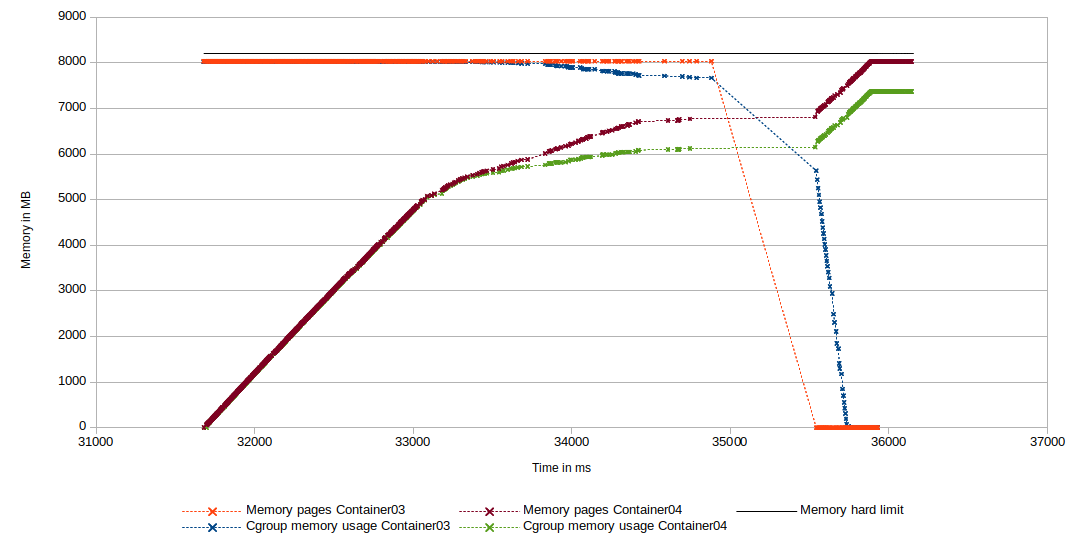
\includegraphics[width=1\linewidth]{pics/010_mem_usage_8200mb_limit_Container03_undContainer04_RDY_FOR_USE_Focus.png}
	\captionof{figure}[Speicher Verbrauch Cgroup 8200MB Limit]{Speicherverbrauch einer Cgroup und Memory-Pages mit Limit von Container03 und Container04 mit \SI{2048000}{mal} malloc(), \SI{60}{\second} sleep(), Fokus}
	\label{fig:010_mem_usage_8200mb_limit_Container03_undContainer04_RDY_FOR_USE_Focu}
\end{minipage}
\vspace{1em}

Container04 verläuft bei der Allokation unter dem gesetzten Limit, siehe Verlauf der dunkelroten und grünen Linie ab ca. \SI{40}{\second} in Abbildung \ref{fig:009_mem_usage_8200mb_limit_Container03_undContainer04_RDY_FOR_USE} nicht wie erwartet. In Abbildung \ref{fig:007_mem_usage_8200mb_limit_Container01_und_Container02_RDY_FOR_USE} war vor der Lücke nur die blau dargestellte Linie der Cgroup von Container01 vom Paging betroffen und die parallel zur grün verlaufende gelbe Linie der Cgroup von Container02 zeigte keine Anzeichen von Paging. Auch an dieser Stelle wird auf den Seiteneffekt, verursacht durch das Paging, nicht weiter eingegangen.

Es wurde gezeigt, dass ein neu ausgeführter Container mit den im Linux-Kernel implementierten Mechanismen in der Lage ist, einen bereits bestehenden Container zu beenden und dann auf dessen Ressourcen zuzugreifen.


